%!TeX root=main.tex

\chapter{روش پیشنهادی برای تشخیص موضع با نظارت}
\thispagestyle{empty}

تغییرات اقلیمی از جمله مهم‌ترین وقایع محیط زیستی عصر حاضر می‌باشد که بر جوامع انسانی تاثیر مستقیمی می‌گذارد. از سوی دیگر با بررسی نظرات کابران در شبکه‌های اجتماعی، می‌توان موضع کلی افراد جامعه نسبت به این موضوع را مورد ارزیابی قرار داد. با پیشرفت تکنیک‌های پردازش زبان طبیعی، امکان تشخیص موضع برای داده‌های شبکه اجتماعی فراهم شده است. برای پیشبرد تحقیقات در این حوزه، رویداد 
\lr{ClimateActivism} (بخش\ref{sec:ClimateActivismStance})
مسئله تشخیص موضع بر داده‌های شبکه‌ اجتماعی توییتر با موضوع تغییرات اقلیمی را برگزار کرد
\cite{thapa2024stance}.

در این پژوهش برای دستیابی به یک مدل هوش مصنوعی برای تشخیص موضع با نظارت، یک روش جستجو جامع به کار گرفته شد. در این جستجو، روش‌های مختلف پیش‌پردازش داده و معماری‌های متفاوت مورد بررسی قرار گرفته است. همچنین تکنیک‌‌های موثر بر مقابله با داده‌های نامتوازن
\LTRfootnote{Imbalance data}،
(مانند افزایش داده و انتخاب تابع ضرر متناسب) نیز استفاده شده است. در نهایت معماری پیشنهادی از ترکیب
\lr{BERTweet}
و شبکه‌ پیچشی
\lr{(CNN)}
و
\lr{Weighted Cross Entropy}
به عنوان تابع ضرر استفاده می‌کند. در ادامه این فصل، روش جستجو استفاده شده، فضا جستجو تعریف شده، جزییات معماری پیشنهادی، آزمایش‌های انجام شده و تحلیل نتایج به صورت مفصل بیان می‌شود.

\section{دادگان آموزشی}
برای آموزش، ارزیابی و مقایسه مدل پیشنهادی از مجموعه داده
\lr{ClimaConvo}\cite{shiwakoti2024analyzing}
استفاده شد. این مجموعه داده شامل شش مسئله مختلف از جمله تشخیص موضع، تشخیص طنز
\LTRfootnote{Humor Detection}
و تشخیص سخنان نفرت انگیز
~\LTRfootnote{Hate Speach Detection}
می‌باشد. در اینجا تنها از بخش تشخیص موضع دادگان استفاده شده است. توزیع داده‌های هر کلاس در جدول
\ref{dataset-statistics}
نشان داده شده است. بخش 
\ref{sec:datasetClimaConvo}
شامل توضیحات تکمیلی درباره مجموعه داده می‌باشد. شکل
\ref{token-len-distribution}
توزیع تعداد تک واژهای مجموعه داده 
\lr{ClimaConvo}
را نشان می‌دهد.
\begin{table}[ht]
	\centering
	\small
	\caption{\label{dataset-statistics} توزیع کلاس‌ها در بخش‌های آموزش، توسعه و ارزیابی مجموعه داده
	\lr{ClimaConvo}}
	
	\vspace{0.2cm}
	\begin{tabular}{ c|c|   c c c}
		\hline
		& \% & موافق & بدون نظر &  مخالف\\
		\hline
		\hline
		آموزش (\lr{Train}) & 70\% & 4328 & 2256 & 700 \\
		توسعه (\lr{Dev}) & 15\% & 897 & 511 & 153  \\  
		ارزیابی (\lr{Test}) & 15\% & 921 & 500 & 141\\
		\hline
		\hline
		مجموع & 100\% & 6146 & 3276  & 994 \\
		\hline
	\end{tabular}
\end{table}


\begin{figure}[H]
	\center{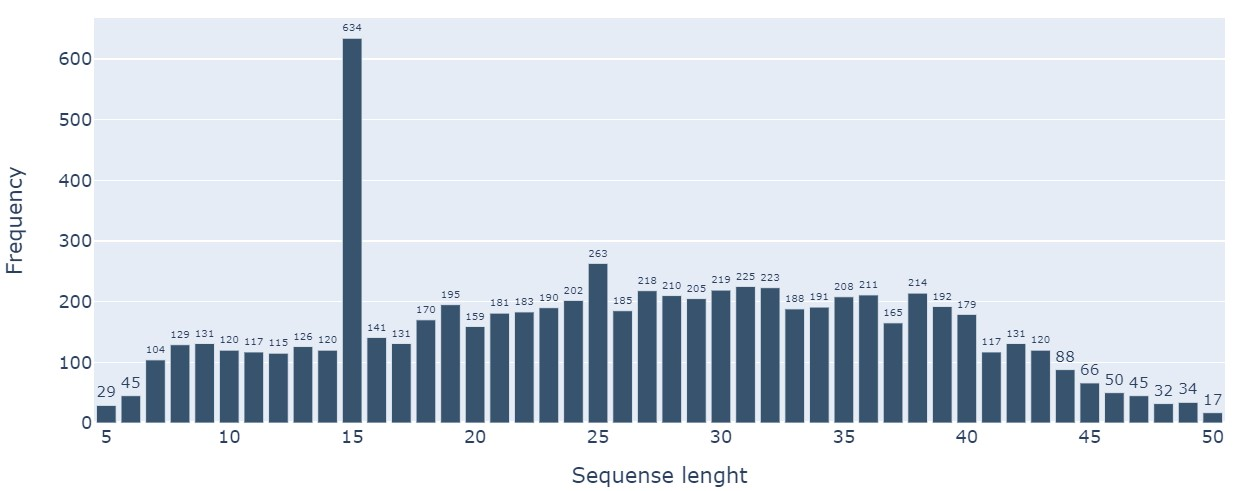
\includegraphics[width=1\linewidth]{images/tolen_len_distribution.jpg}}
	\vspace{-1cm}
	\caption{توزیع تعداد تک واژهای مجموعه داده
	\lr{ClimaConvo} \label{token-len-distribution}}
	
\end{figure}

همچنین در قسمت پایانی این فصل برای ارزیابی عملکرد مدل بر مجموعه داده‌ای که بر روی آن آموزش ندیده، دو بخش "قانونی شدن سقط جنین" و "تغییرات اقلیمی" از مجموعه داده 
\lr{SemEval}\cite{mohammad-etal-2016-semeval}
مورد استفاده قرار گرفت. جدول
\ref{dataset-statistics-semeval}
توزیع کلاس‌های مجموعه داده به ازای هر موضوع را نشان می‌دهد.
\begin{table}[ht]
	\centering
	\small
	\caption{\label{dataset-statistics-semeval} توزیع کلاس‌ها در بخش‌های ارزیابی مجموعه داده
		\lr{SemEval}}
	
	\vspace{0.2cm}
	\begin{tabular}{ c|   c c c}
		\hline
		 موضوع & موافق & بدون نظر &  مخالف\\
		\hline
		\hline
		تغییرات اقلیمی (\lr{CC}) &  11 & 35 & 123 \\
		قانونی شدن سقط جنین (\lr{LA}) &  186 & 45 & 46 \\
		\hline
		\hline
	
	\end{tabular}
\end{table}
\section{روش حل مسئله}
رویکرد ارائه شده، از روش جستجو معماری شبکه عصبی الگو می‌گیرد. بدین منظور معماری شبکه  به چهار بخش اصلی تقسیم شد. به ازای هر یک از بخش‌ها با توجه به دانش قبلی، فضای جستجو متناسب معرفی شد. در ادامه از جستجو تطبیقی برای یافتن بهترین پارامترهای مدل و ابرپارامترها استفاده شد. روش جستجو استفاده شده در مقایسه با جستجو تصادفی و جستجو شبکه‌ای مزایای زیادی دارد. این روش از پیشینه جستجو برای انتخاب پارامترهای بعدی استفاده می‌کند. همچنین در صورت ناموفق بودن یک جستجو، به صورت زودهنگام جستجو را متوقف می‌کند. بنابراین در زمان مناسب می‌تواند جستجو نسبتا جامعی انجام دهد.

از سوی دیگر داده‌های ورودی مدل نیز اهمیت ویژه‌ای دارند. از این رو هفت سطح از پیش‌پردازش داده معرفی شد تا تاثیر آن بر نتایج نهایی مورد بررسی قرار بگیرد. همچنین با توجه به نامتوازن بودن داده‌های آموزشی از  روش‌های افزایش داده برا غلبه به این مشکل استفاده شد.
در ادامه توضیحات مربوط به سطوح پیش‌پردازش داده، روش افزایش داده و رویکرد جستجو معماری به صورت مفصل بیان می‌شود.

\subsection{پیش‌پردازش داده‌ها}\label{sec:preprocess}
آماده‌سازی داده‌های مناسب و با کیفیت یکی از مهم‌ترین بخش‌های آموزش یک مدل یادگیری عمیق است.
ابتدایی‌ترین گام در مسائل پردازش زبان طبیعی، پیش‌پردازش دادە‌ها است که به ارتقاء کیفیت دادە‌ها و استخراج معنای بهتر از آن‌ها کمک می‌کند. پیش‌پردازش دادە‌ها به معنای تمیز کردن و سازماندهی دادە‌های خام به شکل قابل فهم برای آموزش مدل‌های یادگیری عمیق است.

 داده‌های متنی شبکه‌های اجتماعی (همانند توییتر) معمولا شامل نویز و عباراتی هستند که ممکن است مدل را دچار خطا کند. در فرآیند پیش‌پردازش داده‌، رویکرد اصلی این است که هیچ داده‌‌ای دور ریخته نشود و حداکثر اطلاعات از داده‌های متنی موجود استخراج شود. اما به دلیل محدودیت در داده‌های آموزشی، وجود نویز در داده‌ها ممکن است آموزش مدل را با مشکل روبرو کند. در ادامه هفت سطح متفاوت برای پیش‌پردازش داده معرفی می‌شود. روش‌های معرفی شده به صورت سلسله مراتبی هستند. بدین معنا که هر روش نسبت به روش قبلی، اطلاعات بیشتری را حذف می‌کند یا تغییر می‌دهد.
 
\begin{enumerate}
	\item 	\textbf{نگهداشت داده‌های اصلی}:
در این رویکرد فرض کردیم بهترین روش عدم تغییر داده‌های اصلی می‌باشد. در این روش متن داده‌های موجود بدون هیچ تغییری به عنوان ورودی مدل در نظر گرفته می‌شود.
	\item \textbf{ حذف آدرس‌ اینترنتی}
	\LTRfootnote{\lr{URL}}
	: با توجه به اینکه اغلب آدرس‌های اینترنتی به صورت مختصر وجود داشتند (به عنوان مثال
	\href{https://t.co/rs1vhBp2ax}{\lr{https://t.co/rs1vhBp2ax}})
	امکان یافتن الگو از آن‌ها ممکن نبود. بنابراین در این رویکرد فقط آدرس اینترنتی حذف شده و مابقی متن را تغییری نکرد.
	\item حذف نام‌کاربری
	\LTRfootnote{\lr{Username}}:
فرض ما این است وجود نام‌کاربری بدون اینکه اطلاعات دیگری از کاربران داشته باشیم بیشتر موجب گمراهی مدل می‌شود. برای بررسی صحت فرض مطرح شده، این رویکرد را نیز در آزمایش‌های خود قرار دادیم.
	\item حذف همزمان نام کاربری و آدرس اینترنتی:
رویکرد دوم و سوم را برای بررسی اثربخشی همزمان آن‌ها با هم اعمال شد.

	\item حذف همزمان نام کاربری و آدرس اینترنتی و جدا کردن هشتگ: 
	در شبکه‌های اجتماعی همچون توییتر برای بیشتر دیده شدن توییت‌ها و همراهی با رویدادی خاص، گاها هشتگ‌هایی در متن اصلی توییت استفاده می‌شود. استفاده از  هشتگ‌ها جستجو آن‌ها را نیز ساده‌تر می‌کند. در این رویکرد برای تمیز کردن داده‌ها هشتگ‌ها به صورت یک عبارت در آوردیم به گونه‌ای که
 \lr{\texttt{\#FridaysForFuture} }
به
 \lr{\texttt{Fridays For Future}}
 تبدیل می‌شود. انتطار می‌رود بعد از جداسازی هشتگ‌ها عبارت قابل فهم‌تری داشته باشیم.
 
	\item حذف همزمان نام کاربری و آدرس اینترنتی و جدا کردن هشتگ و کوچک کردن حروف:
در زبان انگلیسی معمولا کلمات در ابتدا جمله با حروف بزرگ شروع می‌شوند. از طرفی گاهی کلیه حروف یک کلمه بنا به دلایلی خاص از جمله تاکید، خشم یا عصبانیت به صورت بزرگ نوشته می‌شود. از سوی دیگر دو کلمه
\lr{Book}
و
\lr{book}
هم معنی هستند اما با توجه به اختلاف در حروف اول دو بازنمایی متفاوت در مدل‌های هوش مصنوعی پیدا می‌کنند. یکی از گام‌های پیش‌پردازش داده‌ها کوچک کردن همه حروف
\LTRfootnote{Lower Casing}
می‌باشد. در این سطح از پیش‌پردازش داده قصد داریم تاثیر این عمل بر نتیجه نهایی  مدل را به دست بیاوریم.
	\item تمیز کردن کامل داده‌ها:
	این سطح شامل کامل‌ترین پیش‌پردازش می‌باشد و علاوه بر همه موارد رویکرد ششم، کلمه‌های توقف
	\LTRfootnote{\lr{Stop Words}}
	و علائم دستوری نیز حذف می‌شوند.
\end{enumerate}

در بخش
~\ref{sec:data-cleaning-impact}،
 عملکرد هر یک از روش‌های پیش‌پردازش مورد بررسی قرار می‌گیرد.

\subsection{افزایش داده}\label{sec:dataaug}
یکی از روش‌های استفاده شده برای غلبه بر مشکلات ناشی از مجموعه داده کوچک و نامتوازن، استفاده از تکنیک‌های افزایش داده می‌باشد. در این پژوهش برای افزایش داده، از مدل مبتنی بر
\lr{T5}
که بر روی مجموعه داده‌
\lr{ChatGPT paraphrase}\cite{chatgpt-paraphrases-dataset}
آموزش دیده
\cite{chatgpt-paraphraser}
، برای افزایش داده استفاده می‌کنیم. این مدل آموزش دیده تا متن ورودی را به گونه‌ای دیگر بازنویسی
\LTRfootnote{Paraphrase}
 کند. برای افزایش داده به کمک این روش، توییت‌هایی کلاس مخالف را به عنوان ورودی مدل دادیم. مدل به ازای هر متن، 5 بازنویسی از آن را تولید کرده است. توزیع مجموعه داده آموزشی بعد از افزایش داده در شکل~
 \ref{dataset-distribution}
 قابل مشاهده است. در بخش
 ~\ref{sec:data-aug-impact}،
تاثیر افزایش داده بر نتایج به دست آمده مورد بررسی قرار می‌گیرد.

\begin{figure}[H]
	\center{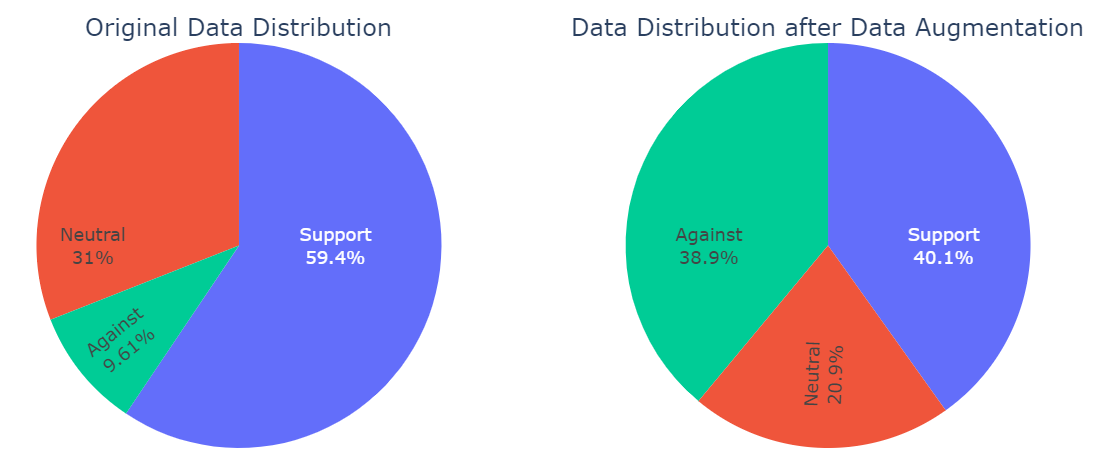
\includegraphics[width=0.8\linewidth]{images/dataset_distribution.png}}
	\caption{توزیع کلاس‌ها قبل و بعد از افزایش داده.}
	\label{dataset-distribution}
\end{figure}
\subsection{جستجو معماری}

در این پژوهش، یک روش جستجو قاعده‌مند
\LTRfootnote{\lr{Systematic}}
 برای یافتن بهترین معماری مدل استفاده شده است. برای تعریف فضا جستجو، ابتدا معماری پیشنهادی به چهار بخش اصلی تقسیم شد. سپس برای هر یک از چهار بخش اصلی فضای جستجو مناسب تعریف شد. برای تعیین مناسب‌ترین پارامترها برای هر بخش، آزمایش‌های متعددی با پیکربندی‌های مختلف انجام داده شد و مقادیر بهینه در فضای جستجوی تعریف‌شده جستجو شد (جدول\ref{Architecture-search-space}). جستجو در فضای تعریف شده با استفاده از کتابخانه
\lr{Optuna} 
، که از نمونه‌بردار با استفاده از الگوریتم 
\lr{TPE (Tree-structured Parzen Estimator) }
استفاده می‌کند، انجام شد. پیکربندی مدل بهینه را بر اساس امتیاز
\lr{Macro-F1} 
در مجموعه توسعه 
\LTRfootnote{Development Set}
انتخاب شد. فضا جستجو تعریف شده برای هر بخش در جدول 
\ref{Architecture-search-space}
قابل مشاهده است.
\begin{table}[h!]
	\centering
	\caption{\label{Architecture-search-space}فضای جستجو معماری پیشنهادی}
	\vspace{0.2cm}
	\begin{tabular}{c  |c }
		\hline
		پارامتر & فضا جستجو\\
		\hline
		بازنمایی کلمات&
		\lr{[BERT, RoBERTa, BERTweet, XLM-RoBERTa, DEBERTA]}\\
		رده‌بند &
		\lr{[FNN, CNN]}
		\\
		\lr{N\_last\_layer} & $[1, 2, 3, 4, 5]$\\
		بهینه‌ساز &
		\lr{[Adam, AdamW, RMSprop, SGD]}
		\\
		تابع ضرر &
		\lr{[Weighted  Cross Entropy, Focal]}
		\\      
		
		
		\hline
		\hline
	\end{tabular}
\end{table}

\begin{enumerate}
	\item بازنمایی کلمات
	\LTRfootnote{Embedding}: برای این بخش تعدادی از مدل‌های کدگذار
\LTRfootnote{Encoder-Only}
که نتایج بهتری در مسائل مشابه کسب کردند را انتخاب کردیم. استفاده از این مدل‌ها در مسائل رده‌بندی
\LTRfootnote{Classification Task}
، متداول‌تر از مدل‌های کدگشا‍~
\LTRfootnote{Decoder-only}
و کدگذار-کدگشا~
\LTRfootnote{Encoder-Decoder}
هستند (جدول~\ref{Architecture-search-space}). 
	\item رده‌بند
	\LTRfootnote{Classifier}:
	در این بخش دو معماری متفاوت را بررسی کردیم.
	\begin{itemize}
		\item معماری شبکه عصبی تماما متصل (FNN)
		\LTRfootnote{Fully Connected Neural Networks}
		
در این بخش	ما از یک معماری سه لایه خطی، به همراه تابع فعال‌سازی 
		\lr{ReLU}و
		\lr{dropout} 
		استفاده ‌می‌کنیم. در نهایت
		\lr{Softmax}
		را بر روی خروجی اعمال می‌کنیم.
				
		\item معماری شبکه عصبی پیچشی (CNN)
		\LTRfootnote{Convolutional Neural Networks}
		
		ایده اصلی معماری استفاده شده مشابه کار سفایا و همکاران
\cite{safaya-etal-2020-kuisail}
		می‌باشد. تفاوت اصلی در این است که به جای 4 لایه آخر، فضا جستجو برای تعداد لایه‌ها تعریف کرده و با آزمایش مقادیر مختلف، بهترین مقدار را به دست می‌آوریم. در این معماری 
		\lr{Embedding} 
		به تعداد 32 فیلتر کانولوشنال موازی با اندازه متفاوت وارد می‌شود (768‍×1، 786×2، 786×3، 786×4، 786×5). معماری پیشنهاد شده مشابه شبکه
		\lr{Inception}
		در بینایی ماشین می‌باشد. بعد از اعمال فیلتر کانولوشنال، تابع فعال‌سازی
		\lr{ReLU}
و 
\lr{Global Max-Pooling}
بر خروجی مرحله قبل اعمال می‌شود. خروجی تولید شده بعد از 
\lr{Faltten}
شدن به یکدیگر
\lr{Concate}
می‌شوند. در انتها با اعمال 
\lr{Softmax}
خروجی نهایی حاصل می‌شود. شکل~\cite{safaya-etal-2020-kuisail} 
معماری رده‌بند متشکل از شبکه عصبی پیچشی را نشان می‌دهد.
		
		
\begin{figure}[H]
	\center{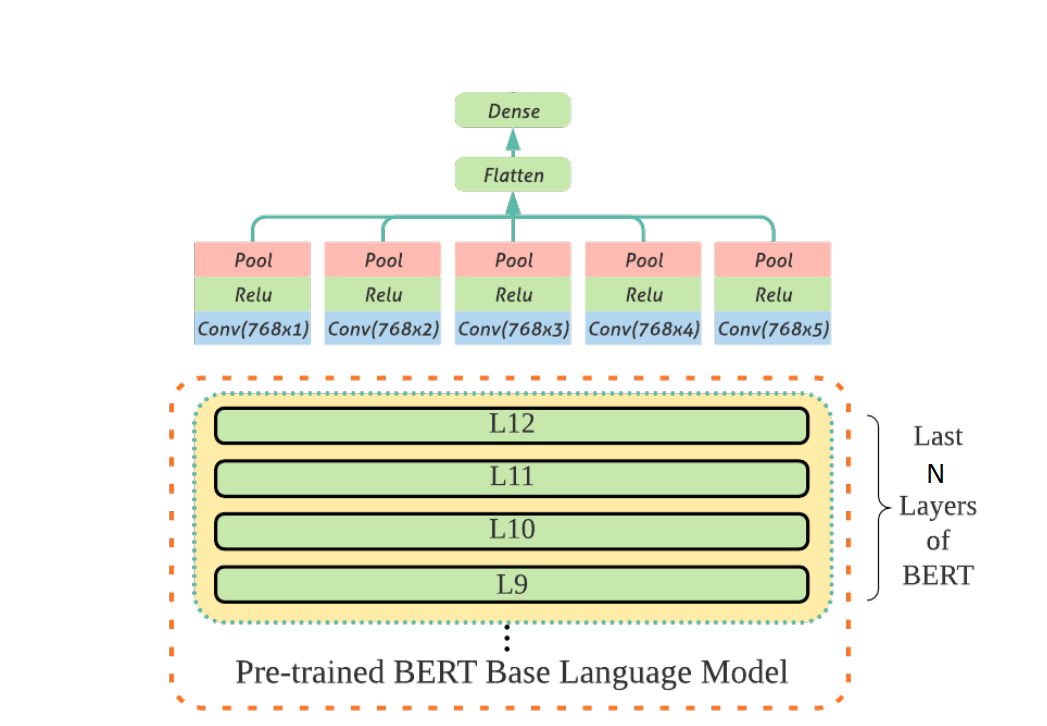
\includegraphics[width=0.7\linewidth]{images/BERT-CNN.PNG}}
	\caption[رده‌بند با شبکه عصبی پیچشی]{رده‌بند با شبکه عصبی پیچشی
\cite{safaya-etal-2020-kuisail}	\label{Bert_CNN}}
\end{figure}
		
	\end{itemize}
	\item بهینه‌ساز
	\LTRfootnote{Optimizer}: فضای جستجو تعریف شده برای بهینه‌سازها شامل چهار بهینه‌ساز معروف، که عملکرد مثبتی از خود نشان دادند، می‌باشد (جدول~\ref{Architecture-search-space}).
	\item تابع ضرر
	\LTRfootnote{Loss Function}:
از‌ آنجایی که با داده‌های نامتوازن و مسئله رده‌بندی مواجه هستیم دو تابع ضرر متفاوت با توجه به شرایط تعریف کردیم.
	
	\begin{itemize}
		\item تابع ضرر
		\lr{Focal}:
		تابع ضرر
		\lr{Focal} \cite{Lin-2017-ICCV}
		با کاهش وزن داده‌های کلاس اکثریت (که به آسانی توسط مدل یادگرفته می‌شوند) در زمان آموزش مدل، تاثیر نامتوازن بودن داده را کم می‌کند. این تابع ضرر به یادگیری صحیح داده‌های سخت‌تر (کلاس اقلیت) تاکید بیشتری دارد تا به این صورت عملکرد نهایی بهبود پیدا کند.
		
		\item تابع ضرر
		\lr{Weighted Cross Entropy}:
		این تابع ضرر گونه‌ای از تابع ضرر استاندارد
		\lr{Cross Entropy}
		می‌باشد به گونه‌ای که به کلاس‌های مختلف، وزن‌های متفاوتی اختصاص می‌دهد. وزن‌های هر کلاس با محاسبه نسبت معکوس تعداد داده‌های آموزشی هر کلاس به کل داده‌های آموزشی به دست می‌آید. به عبارت دیگر اشتباهات کلاس‌ اقلیت نیز اهمیت پیدا می‌کند.
	\end{itemize}
\end{enumerate}

\subsection{انتخاب ابرپارامترها}

انتخاب دقیق ابرپارامترهای استفاده شده در زمان آموزش مدل، از اهمیت ویژه‌ای برخوردار است. در این قسمت از کتابخانه
\lr{Optuna} 
و نمونه‌بردار
\lr{TPE (Tree-structured Parzen Estimator) }
استفاده شد. در این شیوه جستجو ابرپارمترها در هر آزمایش، پارامترها در فضا جستجو انتخاب می‌شوند. این الگوریتم معیاری را برای مقایسه نتیجه آزمایش‌های انجام شده در نظر می‌گیرد. در این پژوهش معیار
\lr{F1-Score}
به عنوان معیار اصلی تعریف شد. در نهایت ترکیبی از فراپارامترها که باعث افزایش معیار 
\lr{F1-Score}
شوند به عنوان پیشنهاد نهایی ارائه می‌شود. همچنین الگوریتم قابلیت خاتمه زودهنگام آزمایش‌هایی با نتایج نامناسب را دارد. جدول
\ref{hyperparam-search-space}
فضای جستجو ابرپارمترهای مدل را نشان می‌دهد.
\begin{table}[h!]
	\centering
	\caption{\label{hyperparam-search-space}فضا جستجو ابرپارامترها}
	\vspace{0.2cm}
	\begin{tabular}{c  |c }
		\hline
		ابرپارامتر & فضای جستجو\\
		\hline
		\lr{Dropout}  &  $[0.1 :  0.5]$\\
		نرخ یادگیری & $[1e^{-5} :  1e^{-2}]$\\
		تعداد دوره
		(\lr{Epoch})&
		$[4, 8]$\\
		اندازه دسته (\lr{Batch Size}) & $[4, 8]$\\
		پارامتر گاما تابع ضرر
		\lr{Focal} & $[1, 2, 3, 4, 5]$\\
		\hline
		\hline
	\end{tabular}
	\centering
\end{table}




\section{آزمایش‌ها و تحلیل نتایج}
برای یافتن بهترین معماری و تحلیل اثرگذاری بخش‌های مختلف بر نتیجه اصلی اقداماتی صورت گرفته است. در این بخش به توضیح اقدامات انجام شده پرداخته می‌شود.

\subsection{گام اول : تحلیل نحوه عملکرد الگوریتم جستجو}

	برای شناخت بیشتر از عملکرد ابزار
	\lr{optuna}
دو آزمایش طراحی و اجرا شد. هدف از انجام این آزمایش‌ها بررسی میزان تکرارپذیری و قابل اتکا بودن این ابزار بود. 
\begin{enumerate}
	\item
	 جستجو در فصای نمونه تعریف شده به ازای هر کدام از روش‌های تمیز کردن داده‌ها 3 بار و هر کدام به تعداد 10 ترایال
	 \footnote{منظور از ترایال همان
	 \lr{trial}
 می‌باشد. آزمایشی که در آن یک بار از فضای جستجو مقادیر پارامترها انتخاب شده و عملکرد مدل بر اساس آن مقادیر مورد بررسی قرار می‌گیرد. در این گزارش برای نزدیک بودن متن نوشته به توضیحات مربوط به 
\lr{optuna}
از همان اصطلاح ترایال استفاده شده است.}
	  تکرار شد (یعنی 10 بار پارامترهای مختلف در فضا جستجو انتخاب شد و مدل آموزش داده شد).  هدف از این بخش بررسی بهترین پارامترهایی است که بعد از 10 بار جستجو  به دست می‌آید. آیا همواره به پارامترهای یکسانی می‌رسد؟
	
	\item
	
	جستجو در فضای نمونه به تعداد ترایال‌های مختلف (10، 20، 40) تکرار شد تا تاثیر افزایش تعداد ترایال بر عملکرد نهایی مدل را به دست بیاید (با مقایسه	
	\lr{F1-Score}).
	
\end{enumerate}

برای جستجو به تعداد ده ترایال، نتایج به دست آمده نشان می‌دهد بهترین پارامترهای پیشنهادی هر کدام از جستجوها تا حدودی با یکدیگر متفاوت بودند. اما 
\lr{F1-Score}
نهایی بهترین مدل تقریبا یکسان بودند. از طرفی با افزایش تعداد ترایال‌ها به 20، نتیجه نهایی بهبود داشت و پارامترهای دقیق‌تری انتخاب شدند. منتها نتایج 40 ترایال و 20 ترایال اختلاف معناداری با یکدیگر نداشتد.

با توجه به نتایج به دست آمده تصمیم گرفته شد آزمایش‌ها را به تعداد 20 ترایال تکرار کرده و بهترین پیکربندی به دست آمده، به عنوان مدل پیشنهادی ارائه شود.

\subsection{گام دوم : به دست آوردن پارامترهای مدل با عملکرد مطلوب  }
در بخش~
\ref{sec:preprocess}
هفت سطح مختلف برای پیش‌پردازش داده‌ها معرفی شد. همچنین در بخش~ 
\ref{sec:dataaug}
نحوه افزایش داده به تفصیل توضیح داده شد. آزمایش‌ها در دو حالت با افزایش داده و بدون افزایش داده تکرار شدند. بنابراین چهارده پیکربندی مختلف تعریف شد. به ازای هر پیکربندی، 20 بار در ترایال‌های مختلف با استفاده از الگوریتم جستجو
\lr{Optuna}
، پارامترهای متفاوتی انتخاب شد و سپس مدل با آن پارامترها آموزش داده شد. همچنین مکانیزمی برای توقف ترایال‌هایی که نتایج آن‌ها در جهت بهبود پیش نمی‌رود نیز وجود دارد. همان‌طور که در بخش‌های قبل اشاره شد، به دلیل بزرگ بودن فضا جستجو، جستجو شبکه‌ای بسیار زمان‌بر و عملا غیر ممکن خواهد بود. برای اینکه بتوان فضای جستجو نسبتا وسیع‌تری را مورد بررسی قرار داد از جستجو تطابقی، که پیشینه جستجو را در انتخاب‌های بعدی در نظر می‌گیرد، استفاده شد. بنابراین در این آزمایش‌ها همه ترکیب‌های ممکن بررسی نشده است اما الگوریتم جستجو به صورت هوشمند در هر ترایال بهترین پارامترها را انتخاب می‌کند و در صورت لزوم ادامه آموزش یک ترایال را متوقف می‌کند. چنین فرآیندی سرعت رسیدن به پارامترهای بهینه را افزایش می‌دهد.
\begin{table*}[h!]
	\centering
	\scriptsize
	\caption[نتایج به دست آمده بر روی مجموعه داده
	\lr{ClimateCanvo Stance} بخش ارزیابی. ]{\label{result}
		نتایج به دست آمده بر روی مجموعه داده
		\lr{ClimateCanvo Stance}
		بخش ارزیابی. روش‌های پیش‌پردازش داده:(
		\lr{C1}: نگهداشت داده‌های اصلی, 
		\lr{C2}: حذف آدرس‌ اینترنتی, 
		\lr{C3}: حذف نام‌کاربری, 
		\lr{C4}: حذف نام کاربری و آدرس اینترنتی به صورت همزمان,     
		\lr{C5}: حذف نام کاربری و حذف آدرس‌ اینترنتی به صورت همزمان و جدا کردن هشتک, 
		\lr{C6}: حذف نام کاربری و آدرس‌ اینترنتی به صورت همزمان و جدا کردن هشتک و کوچک کردن حروف,
		\lr{C7}: تمیز کردن کامل داده‌ها).}
	\vspace{0.2cm}
	\begin{tabular}{c  |c |c c  c  c|c c  c  c}
		\hline
		پیش‌پردازش & افزایش داده &  کدگذار&رده‌بند & تابع ضرر & بهینه‌ساز &
		\lr{F1-Score} & \lr{Recall} & \lr{Precision}& \lr{Accuracy}\\
		\hline
		%report_climate_stance_experiment_on_column_tweet_trial_2
		% , D=0.5 0.68822023
		
		
		\lr{C1} & - &\lr{RoBERTa}&  \lr{CNN(N=1)}& \lr{WCE} & \lr{SGD} &  $71.74$ & $69.94$ & $74.83$& $68.82$\\
		% \tablespace
		\hline
		\hline
		% \tablespace
		%report_climate_stance_experiment_on_column_tweet_remove_url_trial_13 ACC = 0.6491
		% , D=0.2
		\lr{C2} & - & \lr{XLM-RoBERTa}  & \lr{CNN(N=3)}& \lr{WCE} & \lr{AdamW} &  $69.80$ & $69.38$ & $74.16$& $64.91$\\ 
		%report_climate_stance_experiment_on_column_tweet_remove_url_trial_19
		% , D=0.4
		\lr{C2} & - & \lr{BERT}& \lr{CNN(N=2)}& \lr{WCE} & \lr{SGD} &  $70.28$ & $68.64$ & $73.82$ & $66.00$\\
		%report_climate_stance_experiment_on_column_tweet_remove_username_trial_3
		%        0.73815621	0.71894142	0.688951494	0.795527692
		% (D=0.4)
		
		% report_climate_stance_experiment_on_column_data_aug_tweet_remove_url_trial_0
		% 0.701664533	0.687506824	0.662705354	0.752605222
		\lr{C2} & + & \lr{BERT}& \lr{CNN(N=3)} &  \lr{WCE}& \lr{SGD} & $68.75$ & $66.27$ & $75.26$& $70.16$\\
		
		\hline
		\hline
		\lr{C3} & - & \lr{RoBERTa}&  \lr{FNN} & \lr{WCE} & \lr{SGD} & $71.89$ & $68.89$ & $79.55$& $73.81$\\
		
		%report_climate_stance_experiment_on_column_data_aug_tweet_remove_username_trial_4
		\lr{C3} & + & \lr{XLM-RoBERTa} &  \lr{CNN(N=3)} & \lr{F(g=4)} & \lr{SGD} & $68.59$ & $68.51$ & $75.93$& $69.84$\\
		\hline
		\hline
		%report_climate_stance_experiment_on_column_tweet_remove_url_username_trial_0
		% 0.695262484	0.71827397	0.695655047	0.748081657
		% - & - &  - & - &  - & - & -\\
		% , D=0.4
		\lr{C4} & - & \lr{XLM-RoBERTa}  &\lr{CNN(N=2)}&  \lr{WCE} & \lr{RMSprop}&  $71.82$ & $69.56$ & $74.80$ & $69.52$\\
		%trial_2
		%0.728553137	0.723104075	0.696190696	0.769851624
		% , D=0.5
		\lr{C4} & - & \lr{BERT} & \lr{CNN(N=5)} &  \lr{WCE} & \lr{SGD} &  $72.82$ & $69.56$ & $74.80$ & $72.85$\\
		%trial_4
		%0.725992318	0.739746891	0.70919688	0.781799265
		% , D=0.2
		\lr{C4}& - & \lr{XLM-RoBERTa} & \lr{CNN(N=3)} &  \lr{F(g=1)} & \lr{SGD} &  $73.97$ & $70.91$ & $78.17$ & $72.59$\\
		%trial_12
		%0.710627401	0.715227463	0.683140419	0.766553658
		%(D=0.5)
		\lr{C4}& - & \lr{RoBERTa}& \lr{FNN} &  \lr{WCE} & \lr{RMSprop} &  $71.52$ & $68.31$ & $78.17$ & $70.06$\\
		%trial_15
		%0.731754161	0.727294616	0.693864994	0.788514218
		%, D=0.3
		\lr{C4}& - & \lr{XLM-RoBERTa} & \lr{CNN(N=4)} &  \lr{WCE}& \lr{SGD} &  $72.72$ & $69.38$ & $78.85$ & $73.17$\\
		%report_climate_stance_experiment_on_column_data_aug_tweet_remove_url_username_trial_0
		%0.741357234	0.748312045	0.71640203	0.794630353
		
		% C4& \Checkmark &  BERTweet&CNN(\textbf{N=5}) &  \textbf{WCE}&\textbf{SGD} &  \textbf{74.83} &\textbf{ 71.64} &\textbf{ 79.46}&\textbf{74.13}\\
		
		
		\textbf{\lr{C4}}& \textbf{+} &  \textbf{\lr{BERTweet}} & \textbf{\lr{CNN(N=5)}} &  \textbf{\lr{WCE}} & \textbf{\lr{SGD}} & \textbf{\lr{74.47}} & \textbf{\lr{70.31}} & \textbf{\lr{79.31}}& \textbf{\lr{73.11}}\\
		%report_climate_stance_experiment_on_column_data_aug_tweet_remove_url_username_trial_2
		%0.701664533	0.706468713	0.675635533	0.756350482
		
		\lr{C4}& + & \lr{BERT} & \lr{CNN(N=4)} &  \lr{WCE} & \lr{SGD} &  $70.64$ & $67.75$ & $75.63$& $70.01$\\
		
		\hline
		\hline
		% report_climate_stance_experiment_on_column_tweet_remove_url_username_splite_hasghtag_trial_2
		%trial_2
		%0.677336748	0.713373105	0.687480629	0.754339459
		% (D=0.1)
		\lr{C5} & -& \lr{DEBERTA} &  \lr{FNN} & \lr{WCE} & \lr{Adam} &  $71.33$ & $68.78$ & $75.43$ & $67.73$\\
		%trial_5
		%0.721510883	0.727001956	0.6963022	0.771830242
		% , D=0.2
		\lr{C5} & - & \lr{XLM-RoBERTa}  &  \lr{CNN(N=2)} & \lr{WCE}& \lr{SGD} & $72.70$ & $69.63$ & $77.18$ & $72.15$\\
		%trial_10
		%0.715108835	0.72019216	0.68628338	0.774418685
		% (D=0.2)
		\lr{C5} & -&\lr{BERT} &  \lr{FNN} & \lr{F(g=1)} & \lr{SGD} &  $72.01$ & $68.62$ & $77.44$ & $71.75$\\
		
		% report_climate_stance_experiment_on_column_data_aug_tweet_remove_url_username_splite_hasghtag_trial_2
		%0.727272727	0.71209454	0.685105644	0.776805868
		
		\lr{C5} & + & \lr{DEBERTA} &  \lr{FNN} & \lr{WCE}& \lr{AdamW} & $71.20$ & $68.51$ & $77.68$ & $72.72$\\
		
		%report_climate_stance_experiment_on_column_data_aug_tweet_remove_url_username_splite_hasghtag_trial_17
		%0.672215109	0.708500465	0.700169674	0.73417312
		
		\lr{C5} & +& \lr{BERT} &  \lr{CNN(N=3)} & \lr{WCE}& \lr{SGD} &  $70.85$ & $70.01$ & $73.41$ & $67.22$\\
		\hline
		\hline
		
		%report_climate_stance_experiment_on_column_tweet_remove_url_username_splite_hasghtag_lower_case
		%trial_1
		%0.722151088	0.718343626	0.683864994	0.784830121
		% (D=0.4)
		\lr{C6} & - &\lr{BERT}& \lr{FNN}& \lr{F(g=2)} & \lr{SGD} &   $71.83$ & $68.38$ & $74.48$ & $72.21$\\
		%trial_13
		%0.696542894	0.701349897	0.671825906	0.748594973
		% (D=.4)
		\lr{C6} & - & \lr{BERT}& \lr{FNN}& \lr{WCE}& \lr{RMSProp} &  $70.13$ & $67.18$ & $74.85$ & $69.65$\\
		
		%report_climate_stance_experiment_on_column_data_aug_tweet_remove_url_username_splite_hasghtag_lower_case_trial_18
		%0.7285531370038413,0.7270587455031999,0.6943622488660952,0.7856136456290003
		\lr{C6} & + &\lr{XLM-RoBERTa}& \lr{CNN(N=4)}& \lr{WCE}& \lr{SGD} &   $72.70$ & $69.43$ & $78.56$& $72.85$\\
		\hline
		\hline
		%complete_cleaning_trial_4
		%0.717669654	0.716878055	0.687731082	0.765389515
		% , D:0.4
		\lr{C7} & - & \lr{BERT} & \lr{CNN(N=5)} &  \lr{F(g=1)} & \lr{SGD} & $71.68$ & $68.77$ & $76.53$& $71.76$\\
		
		% - & - &  FNN (DropOut=0.5)& roberta  + focal (gamma = 1) + SGD &  71.88 & 68.91 & 79.94\\
		% report_climate_stance_experiment_on_column_data_aug_tweet_complete_cleaning_trial_12
		%0.69206146	0.693698466	0.665635533	0.740977027
		
		\lr{C7} & +  & \lr{BERTweet} & \lr{CNN(N=2)} &  \lr{F(g=4)} & \lr{AdamW} & $69.36$ & $66.56$ & $74.09$ & $69.06$\\
		\hline
		\hline
		
		% - & - &  FNN (DropOut=0.5)& roberta  + focal (gamma = 1) + SGD &  71.88 & 68.91 & 79.94\\
		\hline
		\hline
	\end{tabular}
\end{table*}
نتایج به دست آمده از این جستجو در جدول~
\ref{result}
قابل مشاهده است. در این جدول تنها نتایجی که معیار 
\lr{F1-Score}
بالاتر از 68 درصد کسب کردند، گزارش شدند (از آن‌  جایی که فقط نتایج بیشتر از 68 درصد در معیار
\lr{F1-Score}
گزارش شده است، ممکن است به ازای برخی از حالات پیش‌پردازش داده، رده‌بند
\lr{FNN}
وجود نداشته باشد).




بهترین پارامترهای به دست آمده از این جستجو جامع را به عنوان مدل پیشنهای خود معرفی کردیم. مدل پیشنهادی از 
\lr{BERTweet}
و رده‌بند 
\lr{CNN}
و تابع ضرر 
\lr{Weighted Cross Entropy}
استفاده می‌کند. همچنین برای آموزش مدل، داده‌های آموزشی با تکنیک معرفی شده افزایش داده می‌شود و برای پیش‌پردازش داده‌ها نام کاربری و آدرس اینترنتی را حذف می‌شوند. 
 این روش در رویداد 
\lr{ClimateActivismStance}(بخش \ref{sec:ClimateActivismStance})
توانست بین 19 شرکت‌کننده مسابقات رتبه سوم را کسب کند (جدول
\ref{climate_activism_result}).
جدول
\ref{summery-Result}
نشان می‌دهد معماری طراحی شده توانست مدل پایه
\lr{(Baseline)}
را به 19,97 درصد در معیار
\lr{F1-Score}
بهبود دهد. 
\begin{table}[ht!]
	\centering
	\caption[مقایسه بهترین معماری طراحی شده با مدل پایه.]{\label{summery-Result}
		مقایسه بهترین معماری طراحی شده با مدل پایه. 
		نتایج
		$^*$
		از  
		\cite{shiwakoti2024analyzing}
		گزارش شده است.
	}
\vspace{0.2cm}
	\begin{tabular}{ c   c   c}
		\hline
		\lr{Model} & \lr{ACC} & \lr{F1}  \\
		\hline 
		\lr{BERTTweet} \tablefootnote{رده‌بند
			\lr{CNN}
			با 5 لایه آخر
			\lr{BERTTweet}
			همراه با افزایش داده، تابع ضرر 
			\lr{Weight Cross Entropy}
			و بهینه‌ساز
			\lr{SGD}
			و مکانیزم پیش‌پردازش حذف همزمان نام‌کاربری و آدرس اینترنتی.}
		  & \textbf{$73.11$} & \textbf{$74.47$}  \\
		\lr{XLM-RoBERTa} \tablefootnote{
			رده‌بند
			\lr{CNN}
			با 5 لایه آخر
			\lr{XLM-RoBERTa}،
			تابع ضرر 
			\lr{Focal}
			و بهینه‌ساز
			\lr{SGD}
			و مکانیزم پیش‌پردازش حذف همزمان نام‌کاربری و آدرس اینترنتی.}
		 & $72.59$ & $73.97$ \\
		\lr{ClimateBERT (Baseline)}$^*$ & $65.1$  & $54.5$  \\
		\hline
	\end{tabular}
	
\end{table}

شکل
\ref{metric_per_epoch}
تغییرات معیارهای ارزیابی را به ازای هر دوره از آموزش بر مجموعه داده آموزشی، توسعه و ارزیابی نشان می‌دهد.
\begin{figure}[H]
	\center{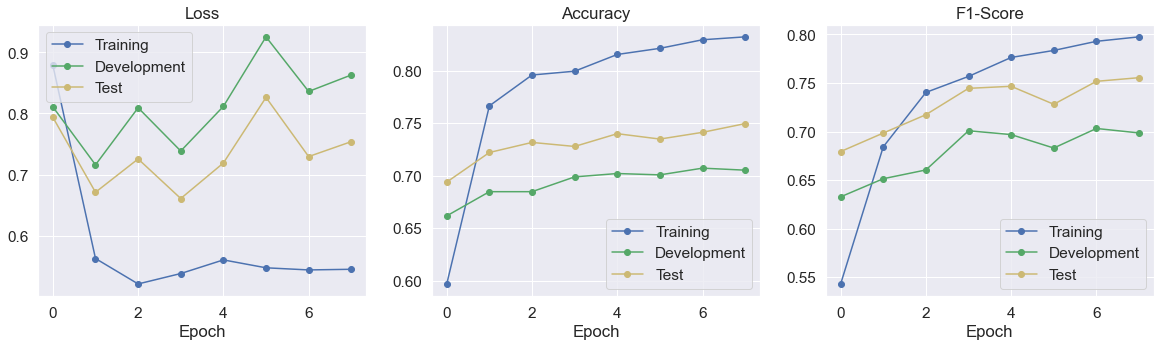
\includegraphics[width=0.9\linewidth]{images/metric_per_epoch.png}}
	\caption{عملکرد مدل آموزش دیده در هر 
	\lr{epoch} آموزش}
	\label{metric_per_epoch}
\end{figure}
در گام بعدی اثربخشی بخش‌های مهم روش پیشنهادی مورد بررسی دقیق‌تر قرار می‌گیرد. به صورت دقیق‌تر ‌تاثیر نوع پیش‌پردازش داده، افزایش دادگان آموزشی، رده‌بند و تابع ضرر بر نتایج نهایی  بررسی  می‌شود.

\subsection{گام سوم : ارزیابی تکمیلی مدل پیشنهادی}
در گام دوم با جستجو کامل بر روی همه پارامترهای مدل و ابرپارامترها، بهترین ترکیب پارامترها به دست آمد. پارامترهای نهایی مدل پیشنهادی در جدول~
\ref{best-config}
قابل مشاهده است. در این بخش با طراحی آزمایش‌هایی سعی شده تا تاثیر هر یک از موارد در نتیجه نهایی به صورت جداگانه بررسی شود.

\begin{table}[h!]
	\centering
	\small
	\caption{\label{best-config}پارامترهای بهترین مدل پیشنهادی.}
	\vspace{0.2cm}
	\begin{tabular}{c  |c }
		\hline
		پارامتر & مقدار\\
		\hline
		تعداد دوره
		 (\lr{Epoch})
	     & $8$ \\
		اندازه دسته (\lr{Batch Size}) & $4$\\
		نرخ یادگیری & $0.007903$\\
		طول عبارت ورودی & $128$ \\
		\lr{Dropout}  &  $0.5$\\
		\lr{Learning schedule} & 
		\lr{Linear Schedule With Warmup}
		\\
		\hline
		کدگذار & 
		\lr{BERTweet}
		\\
		رده‌بند & 
		\lr{CNN}
		\\
		\lr{N\_last\_layer} & $5$\\
		بهینه‌ساز & 
		\lr{SGD}
		\\
		تابع فعال‌سازی&
		 \lr{Weighted Cross Entropy}
		 \\
		\hline
		\hline
	\end{tabular}
	
	\centering
	
\end{table}


\subsubsection{اثربخشی نوع پیش‌پردازش داده}\label{sec:data-cleaning-impact}
برای تعیین میزان اثربخشی نوع پیش‌پردازش بر نتایج به دست آمده، آزمایش‌ها با بهترین پیکربندی تکرار شد (طبق پارامترهای جدول
\ref{best-config}).
در این آزمایش‌ها تنها نوع پیش‌پردارش تغییر کرده و پارامترهای مدل و ابرپارامترها ثابت هستند. برای هر تکنیک پیش‌پردازش، جهت اطمینان از نتایج به دست آمده، آزمایش‌ها 10 بار تکرار شدند. جدول
\ref{data-cleaning-impact}
نتایج به دست آمده را نشان می‌دهد.

\begin{table}[h!]
	\centering
	\small
	\caption[نتایج بررسی اثربخشی نوع پیش‌پردازش داده]
	{\label{data-cleaning-impact}
		نتایج بررسی اثربخشی نوع پیش‌پردازش داده. 
		علامت $\dagger$ نشان می‌دهد نتایج به دست آمده در مقایسه با روش پیش‌پردازش "نگهداشت داده‌های اصلی" به صورت معنی‌دار $(p < 0.005)$ بهتر هستند. علامت $\ast$ نشان‌ می‌دهد نتایج به دست آمده در مقایسه با روش پیش‌پردازش "تمیز کردن کامل داده‌ها" به صورت معنی‌دار $(p < 0.005)$ بهتر هستند.}
	
	\vspace{0.3cm}
	\begin{tabular}{c  |c }
		\hline
		روش پیش‌پردازش &
		 $F1-Score$
		 \\
		\hline
		نگهداشت داده‌های اصلی & $73.98 \pm 0.0012 ^\ast$\\
		حذف آدرس‌ اینترنتی & $73.92 \pm 0.0017 ^\ast$\\ 
		حذف نام‌کاربری & \textbf{$74.35 \pm 0.0015 ^\ast \dagger$} \\
		حذف همزمان نام کاربری و آدرس اینترنتی & $74.11 \pm 0.0029 ^\ast \dagger$\\
		حذف همزمان نام کاربری و آدرس اینترنتی و جدا کردن هشتک & $73.76 \pm 0.0014 ^\ast$\\
		حذف همزمان نام کاربری و آدرس اینترنتی و جدا کردن هشتک و کوچک کردن حروف
		 & $73.72 \pm 0.0009 ^\ast$\\
		تمیز کردن کامل داده‌ها
		 & $72.42 \pm 0.0020 $\\
		\hline
		\hline
	\end{tabular}	
\end{table}

 با ارزیابی مقدار
\lr{F1-Score}
به دست آمده می‌توان نتیجه گرفت روش "حذف نام‌کاربری" و "حذف همزمان نام کاربری و آدرس اینترنتی" در مقایسه با سایر روش‌ها بهترین نتیجه را کسب کردند. همچنین این روش‌ها به صورت معنادار از روش‌های "تمیز کردن کامل داده‌ها" و "نگهداشت داده‌های اصلی" بهتر است. مقدار $p-value$ به دست آمده در مقایسه این روش‌ها با سایر تکنیک‌ها کمتر از $0.0005$ می‌باشد که نشان می‌دهد بهبود معنادار
\LTRfootnote{Significance}
است. همچنین موثرترین روش پیش‌پردازش در مجموعه داده استفاده شده، حذف نام کاربری می‌باشد. علاوه بر این می‌توان گفت همه روش‌ها نسبت به روش "تمیز کردن کامل داده‌ها" نتایج بهتری کسب کردند. این بدان معنی است در این روش‌ ویژگی‌هایی
\LTRfootnote{Feature}
 از ورودی که می‌تواند تاثیر مثبتی بر عملکرد مدل داشته باشد حذف شده است. به عنوان مثال گاهی چندین علامت سوال یا علامت تعجب متوالی (!!!!، ؟؟؟؟؟) نشان دهنده یک حالت خاصی از تعجب یا عصبانیت و یا مخالفت است. اما در روش "تمیز کردن کامل داده‌ها"  با حذف علائم نگارشی، فرصت یادگیری با استفاده از این چنین موارد از مدل سلب می‌شود.

نمودار
~\ref{data-cleaning-impact-chart}
نشان می‌دهد از روش اول (نگهداشت داده‌های اصلی) تا روش سوم (حذف نام‌کاربری) تکنیک‌های پیش‌پردازش باعث بهبود مدل می‌شود. اما بعد از آن هر چه موارد بیشتری از متن ورودی حذف شود، عملکرد مدل به صورت معناداری کاهش می‌یابد. میانگین و بازه اطمینان مدل پیشنهادی در شکل~
\ref{data-cleaning-impact-bar-chart}
را برای انواع تکنیک‌های پیش‌پردازش نشان می‌دهد.

\begin{figure}[H]
	\center{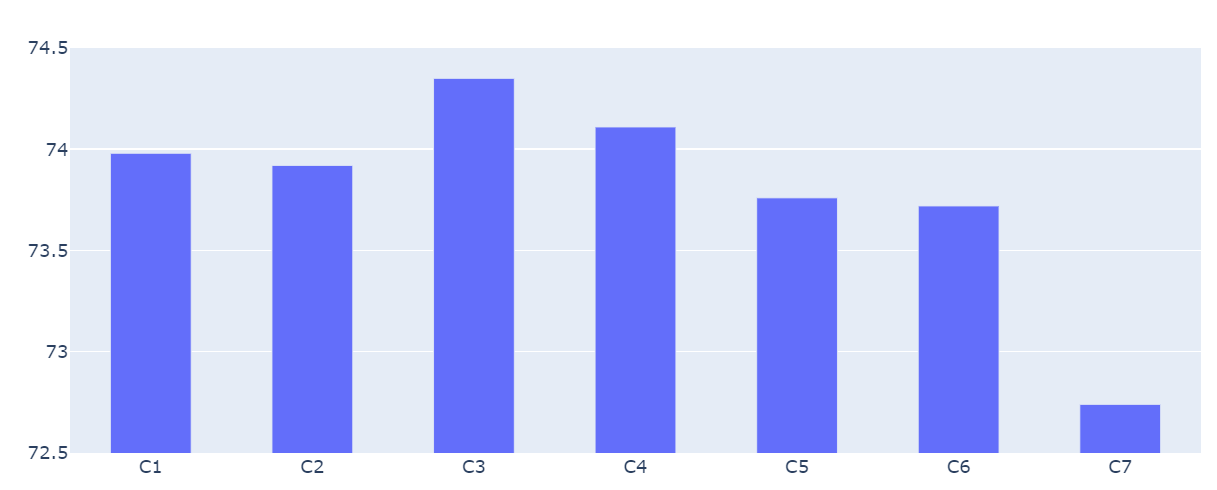
\includegraphics[width=0.9\linewidth]{images/data_cleaning_impact.png}}
	\caption{مقدار
	\lr{F1-Score}
هر یک از تکنیک‌های پیش‌پردازش داده}
	\label{data-cleaning-impact-chart}
\end{figure}

\begin{figure}[H]
	\center{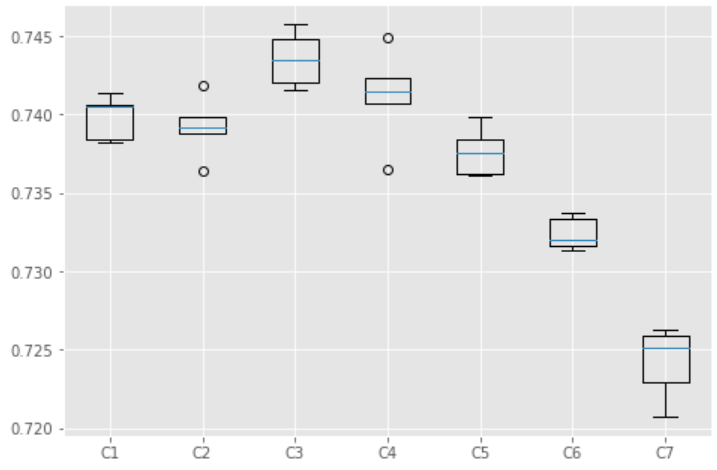
\includegraphics[width=0.6\linewidth]{images/data_cleaning_impact-box-chart-2.png}}
	\caption[بازه اطمینان مدل پیشنهادی بر اساس روش‌های پیش‌پردازش داده]{بازه اطمینان مدل پیشنهادی بر اساس روش‌های پیش‌پردازش داده بر حسب معیار
		\lr{F1-Score}}
	\label{data-cleaning-impact-bar-chart}
\end{figure}

\subsubsection{اثربخشی افزایش داده} \label{sec:data-aug-impact}
افزایش داده یکی از تکنیک‌های بهبود عملکرد مدل در مواجهه با مجموعه داده نامتوازن است. در این آزمایش همه پارامترها و فراپارامترهای مدل یکسان است و تنها داده‌های آموزشی تفاوت دارند. آزمایش‌ها به ازای داده‌های افزایش یافته و داده‌های اصلی 10 بار تکرار شدند. جدول
~\ref{data-aug-impact-table} 
تاثیر افزایش داده‌های آموزشی بر عملکرد نهایی مدل را نشان می‌دهد. بازه اطمینان مدل آموزش دیده با داده‌های افزایش یافته در شکل
~\ref{data-aug-impact-bar-chart}
نمایش داده شده است. همچنین برای بررسی دقیق‌تر، میزان تغییر معیارهای ارزیابی به ازای هر کلاس در جدول
~\ref{data-aug-impact-per-class}
نشان داده شده است. 
\begin{table*}[h!]
	
	\caption[نتایج بررسی اثربخشی افزایش داده. ]
	{\label{data-aug-impact-table}
		نتایج بررسی اثربخشی افزایش داده. علامت $\dagger$ نشان می‌دهد نتایج به دست آمده در مقایسه با حالت بدون افزایش داده به صورت معنی‌دار $(p < 0.05)$ بهتر هستند.}
	\centering
	\vspace{0.2cm}
	\begin{tabular}{c  c |c }
		\hline
		روش پیش‌پردازش&افزایش داده &  $F1-Score$\\
		\hline
		\multirow{2}{*}{حذف نام کاربری}&	-  & $74.11 \pm 0.0029$\\
										&  + & 	$74.79 \pm 0.0036 \dagger$\\
		\hline
		\hline
	\end{tabular}
	
\end{table*}

\begin{figure}[H]
	\center{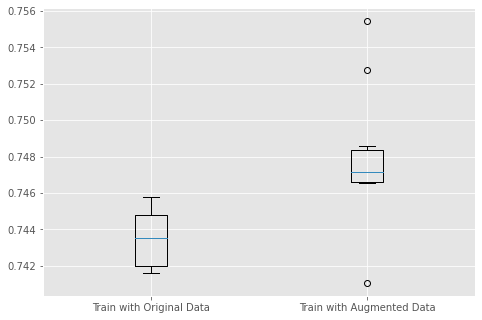
\includegraphics[width=0.6\linewidth]{images/data_aug_impact-box-chart.png}}
	\caption[بازه اطمینان مدل پیشنهادی آموزش دیده با داده‌های افزایش داده‌ شده]{بازه اطمینان مدل پیشنهادی آموزش دیده با داده‌های افزایش داده‌ شده بر حسب معیار
		\lr{F1-Score}}
	\label{data-aug-impact-bar-chart}
\end{figure}

\begin{table}[h!]
	\centering
	\centering
	\caption
	{\label{data-aug-impact-per-class}
		نتایج بررسی اثربخشی افزایش داده به ازای هر کلاس}
	\begin{tabular}{c  c |c c c}
		\hline
		افزایش داده & کلاس & 
		$Precision$ & $Recal$ &$F1-Score$
		\\
		\hline
		
		\multirow{3}{*}{-} & موافق &
		$76.33$ & $78.19$ & $77.25$ \\ 
		& مخالف &
		$75.17$ & $93.80$ & $83.48$ \\ 
		& بدون نظر &
		$62.6$ & $56.90$ & $59.61$ \\ 
		\hline
		\multirow{3}{*}{+} & موافق &
		$81.54$ & $77.58$ & \underline{$79.51$} \\ 
		& مخالف &
		$76.59$ & $95.57$ & \underline{$85.39$} \\ 
		& بدون نظر &
		$59.80$ & $61.16$ & \underline{$60.95$} \\ 
		
		\hline
		\hline
	\end{tabular}
	
	
\end{table}

با بررسی نتایج می‌توان گفت افزایش داده‌های آموزشی عملکرد نهایی مدل را به صورت معناداری بهبود داده است. همچنین با بررسی 
\lr{F1-Score}
به ازای هر کلاس می‌توان گفت پیش‌بینی همه کلاس‌ها نیز بهبود قابل قبولی داشتند. بدین ترتیب مدل با دیدن توزیع مناسبی از داده‌ها در زمان آموزش، عملکرد مناسب‌تری در زمان ارزیابی از خود نشان داده است. همچنین می‌توان نتیجه گرفت تکنیک انتخاب شده برای افزایش داده (بخش
~\ref{sec:dataaug})
داده‌های با کیفیتی تولید کرده است.

\subsubsection{اثربخشی رده‌بند}

در این بخش میزان اثربخشی نوع رده‌بند در عملکرد مدل را مورد بررسی قرار گرفت. از آنجا که طبق نتایج جدول
\ref{data-cleaning-impact}
دو سطح از پیش‌پردازش به صورت معنادار از بقیه روش‌ها بهتر بودند، آزمایش‌های این بخش تنها با دو روش پیش‌پردازش تکرار شد. همچون قسمت قبل، پارامترهای مدل و ابرپارامترها ثابت هستند و تنها نوع رده‌بند تغییر می‌کند. علاوه بر این جهت اطمینان از نتایج به دست آمده، آزمایش‌ها  10 بار تکرار شد. جدول
\ref{classifier-impact}
نتایج به دست آمده را نشان می‌دهد.

\begin{table*}[h!]
	
		\caption[		نتایج بررسی اثربخشی رده‌بند]
	{\label{classifier-impact}
		نتایج بررسی اثربخشی رده‌بند. علامت $\dagger$ نشان می‌دهد نتایج به دست آمده در مقایسه با رده‌بند \lr{FNN} به صورت معنی‌دار $(p < 0.05)$ بهتر هستند.}
	\centering
	\vspace{0.2cm}
	\begin{tabular}{c  c |c }
		\hline
		رده‌بند & روش پیش‌پردازش& $F1-Score$\\
		\hline
		
		\multirow{2}{*}{\lr{CNN}} & حذف نام‌کاربری &\textbf{$74.35 \pm 0.0015 \dagger
			$ } \\ 
				& حذف همزمان نام کاربری و آدرس اینترنتی &
				 $74.11 \pm 0.0029$\\
		\hline
		\multirow{2}{*}{\lr{FNN}} & حذف نام‌کاربری &$73.73 \pm 0.0058$ \\
		 &حذف همزمان نام کاربری و آدرس اینترنتی
		  & $73.91 \pm 0.0045$\\
		
		\hline
		\hline
	\end{tabular}
	
\end{table*}

نتایج نشان می‌دهد رده‌بند ساخته شده با شبکه عصبی پیچشی 
(\lr{CNN})
به صورت معناداری از رده‌بند شبکه عصبی تماما متصل عملکرد بهتری دارد. از آنجا که رده‌بند 
\lr{CNN}
کانولوشن‌هایی با سایزهای مختلف و به صورت موازی اعمال می‌کند، احتمال یادگیری از همسایگی با سایزهای مختلف را پیدا کرده و عملکرد بهتری از خود نشان می‌دهد.
\subsubsection{اثربخشی تابع ضرر}
جدول
\ref{loss-functoion-impact}
تاثیر تغییر تابع ضرر بر نتایج مدل نهایی را نمایش می‌دهد. آزمایش‌های این بخش به ازای هر یک از تنظیمات 10 بار تکرار شدند. سایر پارامترها و اپر پارامترهای مدل ثابت می‌باشد (طبق جدول~
\ref{best-config}).

\begin{table}[h!]
	\centering
	\small

	\caption[نتایج بررسی اثربخشی تابع ضرر بر حسب
	\lr{F1-Score}
	.]{نتایج بررسی اثربخشی تابع ضرر بر حسب
		\lr{F1-Score}. 
	علامت $\dagger$ نشان می‌دهد نتایج به دست آمده در مقایسه با تابع ضرر \lr{Weighted Cross Entropy} به صورت معنی‌دار $(p < 0.05)$ بهتر هستند.
\lr{Cross Entropy}
به اختصار
\lr{CE}
نوشته شده است.
	 	\label{loss-functoion-impact}}
\vspace{0.2cm}
\begin{tabular}{c  |c | c | c}
	\hline
	روش پیش‌پردازش 
	&Focal
	&\lr{Weighted CE}
	& \lr{Weighted CE + Focal}
	\\
	\hline
	نگهداشت داده‌های اصلی &
	$73.95 \pm 0.0034$
	&$73.98 \pm 0.0012$
 	& $74.15 \pm 0.0035$\\

	حذف آدرس‌ اینترنتی &
	$74.03 \pm 0.0011 $
	& $73.92 \pm 0.0017$
	 &  $74.01 \pm 0.0021$
	 \\ 
	حذف نام‌کاربری & 
	$74.13 \pm 0.0015 $
	&\textbf{$74.35 \pm 0.0015$} 
	& $74.31 \pm 0.0031$
	\\
	حذف نام کاربری و آدرس اینترنتی &
	$73.14 \pm 0.0032$
	&$74.11 \pm 0.0029$
	&  $74.35 \pm 0.0025$
	\\
	تمیز کردن کامل داده‌ها&
    $73.12 \pm 0.0028$
	& $72.42 \pm 0.0020 $
	& $73.03 \pm 0.0035 ^\dagger$\\

	\hline
	\hline
\end{tabular}	
\end{table}

همان‌طور که مشخص است استفاده از جمع دو تابع ضرر
\lr{Focal}
و
\lr{Weighted Cross Entropy}
عمکلرد بهتری نسبت به استفاده از یکی از آن‌ها دارد. برای حالت پیش‌پردازش "تمیز کردن کامل داده‌ها" این بهبود معنادار است. در این حالت مقدار $p-value$ به دست آمده کوچکتر $0.05$ می‌باشد. در سایر موارد با مقایسه مقدار
\lr{F1-Score}
می‌توان گفت مدل بهبود داشته اما این بهبود معنی‌دار نمی‌باشد.
\iffalse
\begin{table*}[h!]	
	\caption[ نتایج بررسی اثربخشی پارامتر گاما با روش پیش‌پردازش حذف نام کاربری]
	{\label{focal-gamma-impact}
		نتایج بررسی اثربخشی پارامتر گاما با روش پیش‌پردازش حذف نام کاربری}
	\centering
	\vspace{0.2cm}
	\begin{tabular}{ c |c }
		\hline
		مقدار گاما&
			  $F1-Score$\\
    	\hline
		1 & $74.58$ \\
		2 & $74.14$\\
		3 & $74.01$\\
		4 & \\
		5 & $74.45$\\  
		\hline
		\hline
	\end{tabular}
	
\end{table*}
\fi

\subsubsection{بررسی تاثیر دامنه بر نتایج مدل آموزش دیده}
یکی دیگر از بررسی‌های صورت گرفته میزان 
\lr{Domain Specefic}
بودن مدل آموزش دیده می‌باشد. برای بررسی دقیق‌تر، دو موضوع تغییرات آب‌ و هوایی و قانونی شدن سقط جنین از مجموعه داده
\lr{SemEval-2016}
انتخاب شدند. به این منظور مدل‌های آموزش دیده بر روی مجموعه داده 
\lr{ClimaConvo}
بر دو قسمت از مجموعه داده 
\lr{SemEval2016}
مورد ارزیابی قرار گرفتند. نتایج به دست آمده در جدول~
\ref{domain-specefic}
قابل مشاهده است.

\begin{table}[h!]
	\centering
	\small
	\caption
	{\label{domain-specefic}
		بررسی تاثیر دامنه بر نتایج مدل آموزش دیده بر اساس معیار
		\lr{F1-Score}.}
	\vspace{0.2cm}
	\begin{tabular}{ c | c |c | c}
		\hline
		روش پیش‌پردازش & 
		\lr{ClimaConvo}
		&\lr{SemEval-CC}
		& \lr{SemEval-LA}
		\\
		\hline
		نگهداشت داده‌های اصلی &
		$73.98 \pm 0.0012$&
		$30.89 \pm 0.0216$ &
		$29.65 \pm 0.0142$\\
		
		حذف آدرس‌ اینترنتی &
		$73.92 \pm 0.0017$
		& $29.97 \pm 0.0231$
		& $31.05 \pm 0.0074$ \\ 
		حذف نام‌کاربری & 
		\textbf{$74.35 \pm 0.0015$} 
		& $30.53 \pm 0.0215$
		& $29.11 \pm 0.0104$
		\\
		حذف همزمان نام کاربری و آدرس اینترنتی & 
		$74.11 \pm 0.0029$
		& $30.34 \pm 0.0187$
		& $30.40 \pm 0.0088$
		\\
		تمیز کردن کامل داده‌ها
		& $72.42 \pm 0.0020 $
		& $30.18 \pm 0.0328 $
		& $29.05 \pm 0.0142 $
		\\
		
		\hline
		\hline
	\end{tabular}	
\end{table}

در مجموعه داده 
\lr{SemEval}
تاثیر نوع پیش‌پردازش کمتر می‌باشد. همچنین موضوع مجموعه داده
\lr{ClimaConvo}
و 
\lr{SemEval-CC}
یکسان است اما عملکرد مدل بر روی آن بسیار ضعیف است.  به نظر می‌رسد گذر زمان باعث شده مدل آموزش دیده بر روی مجموعه داده 
\lr{ClimaConvo}
بر مجموعه داده 
\lr{SemEval-CC}
عملکرد مناسبی نداشته باشد. به عبارت دیگر گذر زمان موجب تغییر در نوع داده‌ها شده و بنابراین مدل آموزش دیده بر داده‌های جدید (جمع‌آوری شده در سال 2022)  مناسب داده‌های قدیمی جمع‌آوری شده (در سال 2016) نمی‌باشد.
از طرف دیگر عملکرد مدل بر موضوع قانونی شدن سقط جنین چندان مناسب نیست. به طور کلی می‌توان گفت مدل برای داده‌های با موضوع و توزیع متفاوت نمی‌تواند عملکرد مناسبی داشته باشد. 
\subsection{تحلیل خطا}
با تحلیل خروجی به دست آمده می‌توان گفت مدل در پیشبینی کلاس بدون نظر ضعیف است. شکل
\ref{confusion_matrix}
نشان می‌دهد که در در 209 نمونه کلاس موافق به اشتباه بدون نظر پیشبینی شده است. همچنین در 149 نمونه کلاس بدون نظر به اشتباه موافق پیشبینی شده است. همچنین گاهی در عبارات کلاس مخالف که در قالب طعنه یا کنایه مطرح شده، مدل در تشخیص کلاس درست دچار خطا میشد. در این نوع توییت، نویسنده متن با کنایه مخالفت خود را نسبت به موضوع اهمیت تغییرات اقلیمی بیان می‌کند. در حالی که مدل نتوانسته بود این موضوع را به درستی درک کند. در جدول
\ref{error-example}
نمونه‌ای از اشتباهات در خروجی قابل مشاهده است.


\begin{figure}[H]
	\center{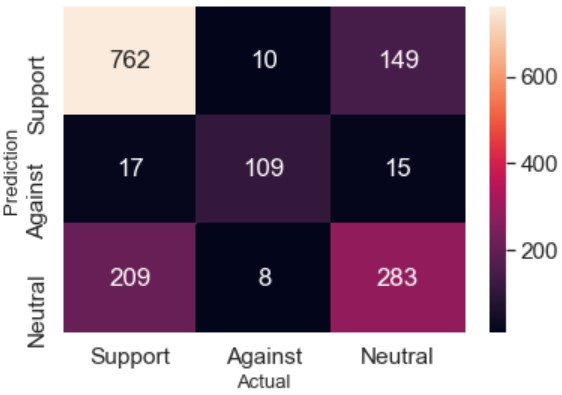
\includegraphics[width=0.5\linewidth]{images/confusion_matrix.jpg}}
	
	\caption{ماتریس درهمریختگی برای داده ارزیابی مجموعه
		\lr{ClimaConvo}}
	\label{confusion_matrix}
\end{figure}

\begin{table}[h!]
	\small
	\caption{چند نمونه  پیشبینی‌های اشتباه مدل}
	\label{error-example}
	\centering
	\vspace{0.2cm}
	\begin{tabular}{c | c c c}
		\lr{\ }
		متن توییت & نوع خطا & کلاس اصلی & کلاس پیش‌بینی شده
		\\
		\hline
		
		\begin{tabular}{@{}c@{}}
			\lr{\#FridaysForFuture \#ClimateChange\#ExtinctionRebellion} \\ 
			\lr{\#GlobalWarming What are we saving?}\\
		\end{tabular}
		& کنایه & مخالف& بدون نظر
		\\
		\hline
		\hline
	\end{tabular}
	
\end{table}

برای بررسی کامل‌تر علت خطاهای مدل، با استفاده از ابزار
\lr{Transformers Interpret} \LTRfootnote{\href{https://github.com/cdpierse/transformers-interpret}{https://github.com/cdpierse/transformers-interpret}}
تحلیلی از خروجی تولید شده توسط مدل صورت گرفت. شکل
\ref{error-analysis}
دو مثال از پیشبینی صحیح مدل را نشان می‌دهد. رنگ سبز نشان‌ می‌دهد که برای پیش‌بینی کلاس نهایی، توجه بیشتری به آن کلمه شده است. نکته قابل توجه این است که برای هر دو خروجی مدل توانسته به کلمات تاثیرگذار توجه کند. به عبارت دیگر مدل کلمات مهم و تاثیرگذار برای فهم متن را توانسته به درستی تشخیص دهد. بنابراین همان‌طور که انتظار می‌رفت پیشبینی مدل نیز صحیح می‌باشد.  در مقابل گاهی کلمات مورد توجه مدل برای پیشبینی صحیح کافی نیست. به عبارت دیگر نیاز به فهم بیشتری دارد. در شکل
\ref{error-analysis-wrong-answers}
دو نمونه از پیشبینی نادرست مدل مشاهده می‌شود. در مثال دوم اگر کلمات
\lr{dying}
و 
\lr{don't care}
نیز مورد توجه مدل قرار می‌گرفت، احتمال پیشبینی درست توسط مدل افزایش می‌یافت.

\begin{figure}[H]
	\center{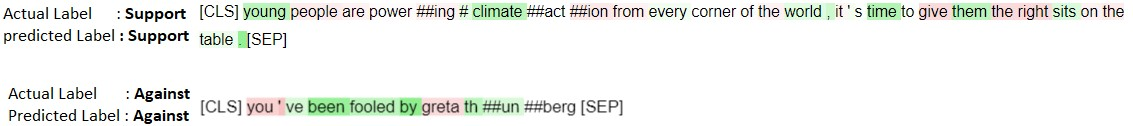
\includegraphics[width=1\linewidth]{images/TransformersInterpretTruePredictedLabel.jpg}}
    \vspace{-1cm}
	\caption{خروجی میزان توجه مدل به کلمات ورودی برای پیشبینی‌های درست}
	\label{error-analysis}
\end{figure}

\begin{figure}[H]
	\center{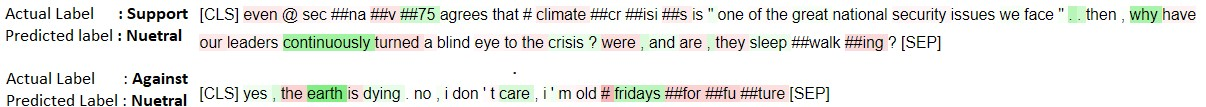
\includegraphics[width=1\linewidth]{images/TransformersInterpretFalsePredictedLabel.jpg}}
	\vspace{-1cm}
	\caption{خروجی میزان توجه مدل به کلمات ورودی برای پیشبینی‌های اشتباه}
	\label{error-analysis-wrong-answers}
\end{figure}


\subsection{مزایا و معایب روش پیشنهادی}
روش پیشنهادی حل مسئله شامل یک تکنیک گام به گام برای طراحی معماری پیشنهادی و بررسی اثربخشی آن است. با توجه به فضای جستجو بررسی شده، می‌توان گفت این روش توانست به نتایج بسیار قابل قبولی دست پیدا کند. همچنین تعریف فضای جستجو به صورت مناسب نیز از دیگر دلایل موفقیت روش پیشنهادی است (استفاده از 
\lr{CNN}
در رده‌بند). از سوی دیگر بررسی انواع پیش‌پردازش متن در اکثر پژوهش‌ها مورد غفلت واقع می‌شود. اما مزیت این پژوهش توجه به روش پیش‌پردازش و برررسی انواع آن است.

از جمله معایب روش ارائه شده نیاز به داده آموزشی کافی برای آموزش مدل می‌باشد. از طرف دیگر طبق بررسی‌های انجام شده، مدل آموزش دیده
\lr{Domain Specific}
می‌باشد و عملکرد مناسبی در سایر دامنه‌ها که در آن آموزش داده نشده، از خود نشان نداده است. وجود 
\lr{GPU}
با رم مناسب برای آموزش مدل‌ها ضروری است.



\subsection{نحوه پیاده‌سازی و اجرا آزمایش‌ها}
پیاده‌سازی پروژه در 
\href{https://github.com/ghazaleh-mahmoodi/Climate_Activism_Stance_Detection}{اینجا}
\LTRfootnote{\href{https://github.com/ghazaleh-mahmoodi/Climate_Activism_Stance_Detection}{https://github.com/ghazaleh-mahmoodi/Climate\_Activism\_Stance\_Detection}}
قابل مشاهده می‌باشد که با زبان پایتون و فریم‌ورک پارتورچ انجام شده است. برای اجرا آزمایش‌ها لازم است با دستور 
\lr{pip3 install -r requirements.txt}
پکیج‌های مورد نیاز برای اجرا کد را نصب کنید. با توجه به طولانی بودن زمان اجرا کل آزمایش‌ها بهتر است با دستور 
\lr{screen}
یک اسکرین جدید برای اجرا بسازید و به شکل معمول دستورات را اجرا کنید. در این صورت حتی با بستن ترمینال اجرا ادامه پیدا می‌کند. با
\lr{screen -r}
در صورت باز کردن مجدد ترمینال می‌توانید فرآیند و میزان پیشرفت اجرا را ببینید.
راه حل دیگر برای تداوم اجرا در صورت بستن ترمینال استفاده از دستور 
\lr{nohup}
است. کافیست
\lr{nohup bash stance\_run.bash}
را اجرا کنید. خروجی‌های اجرا در 
\lr{nohup.out}
قابل مشاهده می‌باشد.
\newline
در صورتی که یک
\lr{screen}
جدید برای خود ساختید، با دستور
\lr{bash stance\_run.bash}
کلیه آزمایش‌ها به صورت متوالی اجرا می‌شود. در نهایت نتایج به دست‌آمده در پوشه 
\lr{result}
ذخیره می‌شود. همچنین وزن‌های شبکه در پوشه
\lr{models}
قابل مشاهده می‌باشند.
\newline
برای اجرا از سخت‌افزار
\lr{GPU.1080Ti.xlarge}
با رم 
\lr{31.3GB}
استفاده شد. دستور 
\lr{nvidia-smi}
میزان استفاده از 
\lr{GPU}
را نمایش می‌دهد. خروجی این دستور در هنگام آموزش مدل به صورت شکل \ref{nvidia-smi} شد.
\begin{figure}[H]		  		    			  	 \center{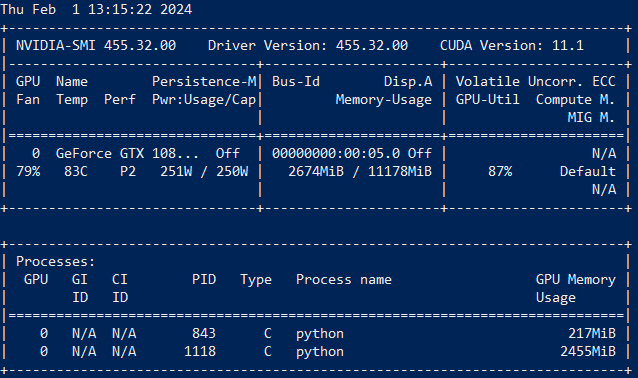
\includegraphics[width=0.8\linewidth]{images/nvidia-smi.jpg}}
	\caption{میزان مصرف \lr{GPU}در زمان آموزش مدل پیشنهادی}
	\label{nvidia-smi}
\end{figure}

\section{جمع‌بندی}
در این فصل به مسئله تشخیص موضع با نظارت پرداخته شد. ابتدا مجموعه داده‌های مورد استفاده معرفی شدند. در ادامه روش حل مسئله شامل تعریف اتولع حالات پیش‌پردازش داده، نحوه افزایش داده، روش جستجو برای معماری و ابرپارامترها و مثادیر فضای جستجو به صورت مفصل بیان شد. در انتها برای بررسی تاثیر نحوه پیش‌پردازش، افزایش داده، رده‌بند و تابع ضرر آزمایش‌های اصولی طراحی و انجام شد. در فصل بعد به مسئله تشخیص موضع بدون داده آموزشی پرداخته می‌شود.

